\documentclass[12pt, a4paper]{article}

\usepackage[utf8]{inputenc}
\usepackage[T1]{fontenc}
\usepackage[francais]{babel}
\usepackage[top=2cm, bottom=2cm, left=2cm, right=2cm]{geometry}
\usepackage{verbatim}
\usepackage{graphicx}
\usepackage{listings}
\usepackage[dvipsnames]{xcolor}
\lstset{
%upquote=true,
columns=flexible,
basicstyle=\ttfamily,}

\title{Projet IHM -- Rapport 2 -- RICM4}
\author{\bsc{Fréby} Rodolphe -- \bsc{Barbier} Jérome -- \bsc{Husson} Augustin -- \bsc{Labat} Paul}
\date{\today}



\begin{document}
\maketitle
\tableofcontents
\newpage

\textcolor{Violet}{\section{Introduction}}
Dans ce second rapport, nous décrirons l'activité que devra permettre notre prototype, au travers de scénarios d'usages, modèle de tâches.

\textcolor{Violet}{\section{Scénarios d'usages}}
\textcolor{NavyBlue}{\subsection{Scénario 1 - Bob, un utilisateur novice}}


Bob est un utilisateur novice et il décide d'utiliser CTTE pour la première fois. Au lancement du logiciel, une fenêtre pop-up s'affiche lui demandant s’il désire suivre un tutoriel pas à pas pour apprendre à manier le logiciel. Cependant, il n'a pas le temps nécessaire, donc il décide de la fermer pour immédiatement tenter de réaliser ce qu'il souhaite. Il va donc tenter de comprendre rapidement l'utilisation des différentes fonctionnalités du logiciel, en passant sa souris au travers des menus et sur les boutons pour obtenir des informations.\\ 


Par la suite, il décide de cliquer sur le nœud déjà présent dans la zone de travail, afin de voir comment réagit le logiciel. Il remarque alors que la zone de travail située sous les boutons principaux de gestion se met à jour, lui donnant une liste de champs définissant le nœud en question. Il décide donc de modifier les champs à sa convenance, afin de mettre à jour les données pour qu'elles correspondent à ses désirs.\\


Bob explore par la suite le dernier menu sur la gauche, afin d'obtenir des informations sur les icônes présentes. De suite, il remarque qu'il peut créer de nouveaux nœuds, et clique sur l'un d'eux, celui qui correspond au mieux à ce qu'il recherche d'après les infobulles. Le nouveau nœud ainsi créé se place en dessous du précédent. Il le sélectionne et met à jour les informations comme pour le nœud précédent. \\


Mais il a toujours besoin de créer de nouveaux nœuds, il va donc répéter l'opération, et remarquer que le nouveau nœud se place à la suite de celui qui est sélectionné dans la zone de travail. Il décide donc de le supprimer, car celui-ci ne se situe pas là où il le désire.\\


Après quelques minutes de travail, son téléphone sonne, et on lui demande de se déplacer pour aller chercher sa fille au cinéma. Il décide donc de sauvegarder son travail avant de partir, pour cela il décide de cliquer sur le menu \emph{File}, puis \emph{Save as}. Une fois la sauvegarde terminée, il ferme le logiciel, celui lui demande s’il veut sauvegarder avant de quitter, Bob choisi non, et s'absente.\\

\newpage
\begin{figure}[h]
\begin{center}
   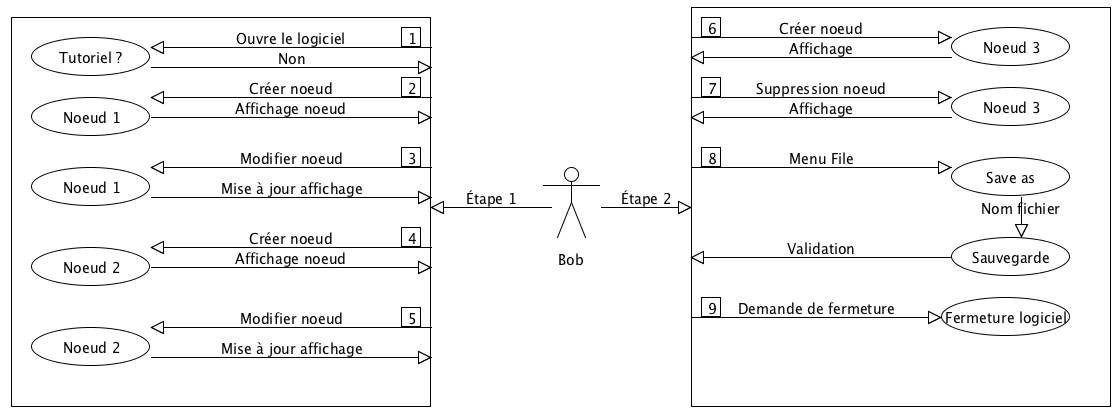
\includegraphics[scale = 0.43]{scenario-bob.png}
	\caption{Le scénario de Bob}
	\end{center}
\end{figure}

\textcolor{NavyBlue}{\subsubsection{Analyse}}

Tout d'abord, à l'ouverture, une boîte de dialogue va s'ouvrir pour signaler que c'est la première ouverture, et va demander si l'utilisateur veut un tutoriel. En cliquant sur non, la boîte de dialogue va simplement se fermer (1).\\ 


Ensuite, en cliquant sur le bouton d'ajout d'un nœud, le système va vérifier si l'action est possible. Si ça l'est, le nœud est ajouté, sinon un message d'erreur est fourni (2).\\ 


A la modification d'un nœud, lors de la validation, le système va s'assurer que la modification est possible, l'effectuer puis fournir une boîte de dialogue comme confirmation, sinon un message d'erreur apparaitra (3).\\  


L'étape suivante reprend le principe de l'étape 2 (4) puis de l'étape 3 (5), de même, le nœud suivant est créé suivant le principe de l'étape 2 (6).\\ 


Lors de la suppression, l'utilisateur va sélectionner le nœud voulu, un marqueur va le lui indiquer, puis il va cliquer sur \emph{Delete}. Le nœud va ainsi être supprimé de l'affichage et du système, ou un message d'erreur sera renvoyé dans le cas contraire (7).\\ 


L'utilisateur va ensuite cliquer sur \emph{File}, qui va ouvrir le menu, puis cliquer sur \emph{Save as}, et rentrer son nom de fichier voulu, puis faire \emph{OK}. Si le fichier existe déjà, une boîte de dialogue demandera confirmation de sauvegarde, sinon le fichier est sauvegardé (9).\\ 


A la demande de fermeture, le logiciel ouvrira une boîte de dialogue pour demander si l'utilisateur (Bob) souhaite enregistrer son travail avant de fermer complètement le logiciel. En cliquant sur \emph{Oui} (quitter sans sauvegarder), le logiciel se fermera simplement (10). \\ \newpage
\textcolor{NavyBlue}{\subsection{Scénario 2 - Alice, une utilisatrice experte}}


Alice arrive au travail à 8 h 15, légèrement en retard, elle décide donc de reprendre immédiatement ce qu'elle a commencé hier. Elle lance CTTE, et une fois lancé, fait la commande \emph{CTRL + o} afin d'ouvrir son document. Elle rajoute des tâches et les modifie à sa convenance, en effectuant des sauvegardes rapides par \emph{CTRL + s}. Elle décide également de faire une sauvegarde en temps que \emph{JPG}, pour cela elle clique sur \emph{File}, puis \emph{Save as}, puis \emph{Save as JPG} \\


Ses collègues de travail l'appel pour un café, elle décide de fermer le logiciel le temps de son absence, pour cela elle effectue la commande \emph{CTRL + Q}. Le logiciel lui signale qu'il va être fermé, et lui demande si elle désire sauvegarder son travail. Elle clique sur non, puis s'absente.\\

\begin{figure}[h]
\begin{center}
   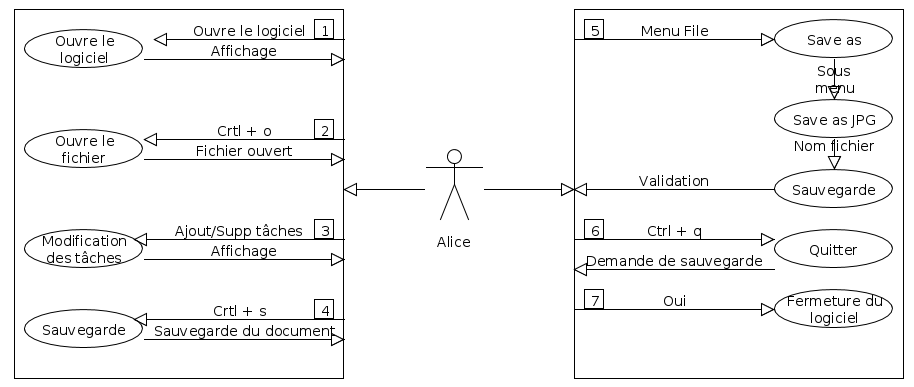
\includegraphics[scale = 0.52]{scenario-alice.png}
	\caption{Le scénario d'Alice}
	\end{center}
\end{figure}

\textcolor{NavyBlue}{\subsubsection{Analyse}}

A l'ouverture du logiciel, Alice se retrouve directement en face de l'interface de travail, sans avoir la demande du tutoriel, car ce n'est pas la première fois que le logiciel est lancé (1).\\


En effectuant le raccourci clavier \emph{CTRL + o}, le logiciel ouvre la boîte de dialogue d'ouverture de fichier. Au moment de valider, le système vérifie que le fichier soit ouvrable, s’il est cela s'affiche sur l'interface, sinon une erreur est renvoyée par une boîte de dialogue (2).\\


Par la suite, l'utilisation de l'ajout ou la suppression des tâches fonctionne comme dans le scénario précédent (3).\\


Au moment de taper \emph{CTRL + s}, le logiciel sauvegarde sur le fichier qui a été ouvert le travail effectué, et grise le bouton (4). \\


Alice souhaite ensuite enregistrer le fichier en \emph{JPG}. Pour cela, elle clique sur \emph{File} qui lui ouvre le menu, elle se rend ensuite dans le sous-menu \emph{Save as} afin de faire \emph{Save Tree as JPG}. Une boîte de dialogue de sauvegarde s'ouvre alors, fonctionnant comme les boîtes de dialogues de sauvegarde précédentes (5).\\


Au moment où elle fait \emph{CTRL + q}, le logiciel va ouvrir la boîte de dialogue de fermeture et demander si elle veut quitter sans sauvegarder. En cliquant sur \emph{oui}, le logiciel se ferme sans sauvegarder (6).


\textcolor{NavyBlue}{\subsection{Scénario 3 - Ève, une utilisatrice familière avec le logiciel}}


Ève décide de modifier un document existant. Pour cela, elle clique sur le bouton \emph{open} afin de pouvoir charger son document. Une fois le document chargé, elle le modifie à sa guise, en cliquant sur le bouton propriété. Elle décide de le sauvegarder en cliquant sur l'icône correspondante.\\


Cependant, elle ne se rappelle plus d'une manipulation particulière. Elle décide de cliquer sur \emph{Help} et d'ouvrir le menu de recherche dans l'aide. Une fois cela effectué, elle décide d’effectuer une recherche sur un nœud en particulier. Pour cela, elle utilise la fonction recherche en bas à gauche de l'interface. \\


Elle décide par la suite de zoomer sur le résultat de sa recherche, à l'aide de l'icône correspondante. Elle clique de nouveau sur propriété, et modifie ce qu'elle souhaite. Elle clique ensuite sur la croix rouge afin de fermer le logiciel. Elle se rend compte qu'elle a oublié de le sauvegarder, grâce au message fourni par le logiciel. Elle décide de cliquer sur oui, puis sauvegarde son document avant de fermer le logiciel.

\begin{figure}[h]
\begin{center}
   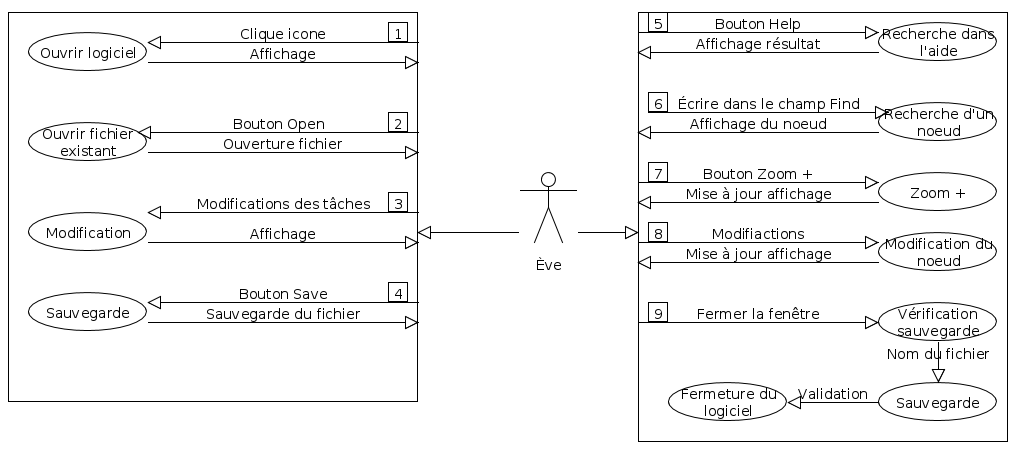
\includegraphics[scale = 0.47]{scenario-eve.png}
	\caption{Le scénario d'Ève}
	\end{center}
\end{figure}

\newpage
\textcolor{NavyBlue}{\subsubsection{Analyse}}

De la même manière que les scénarios précédents, elle lance le logiciel, qui n'affiche pas le tutoriel (ce n'est pas le premier lancement) (1). \\


Elle clique sur le bouton \emph{open}, qui va lui ouvrir la boîte de dialogue de choix de fichier à ouvrir et qui se comporte comme dans le scénario précédent (2).\\


Une fois son travail ouvert, elle modifie le document comme l'a fait Alice en étape 3 (3).\\


Elle clique ensuite sur le bouton \emph{Save}, qui va automatiquement sauvegarder le fichier en écrasant celui par lequel le travail a été ouvert (4), et griser le bouton. \\


Elle clique ensuite sur le menu d'aide, puis sélectionne la fonction de recherche dans l'aide. Une boîte de dialogue se présente donc, dans laquelle elle effectue sa recherche. Une fois la recherche effectuée, elle ferme la boîte de dialogue (5).\\ 


Au moment de cliquer sur la loupe +, le logiciel va agrandir la zone de travail d'un pas prédéfini, centré sur le centre de la fenêtre de travail (7).\\


Elle effectue des modifications comme précédemment, l'affichage se met à jour en conséquence (8).\\


Enfin, elle ferme le logiciel en cliquant sur la croix rouge, qui ouvre la boîte de dialogue lui demandant si elle souhaite quitter sans sauvegarder. En faisant \emph{oui}, le logiciel se ferme (9).
\newpage
\textcolor{Violet}{\section{Modèle des tâches}}

\begin{figure}[h]
\begin{center}
   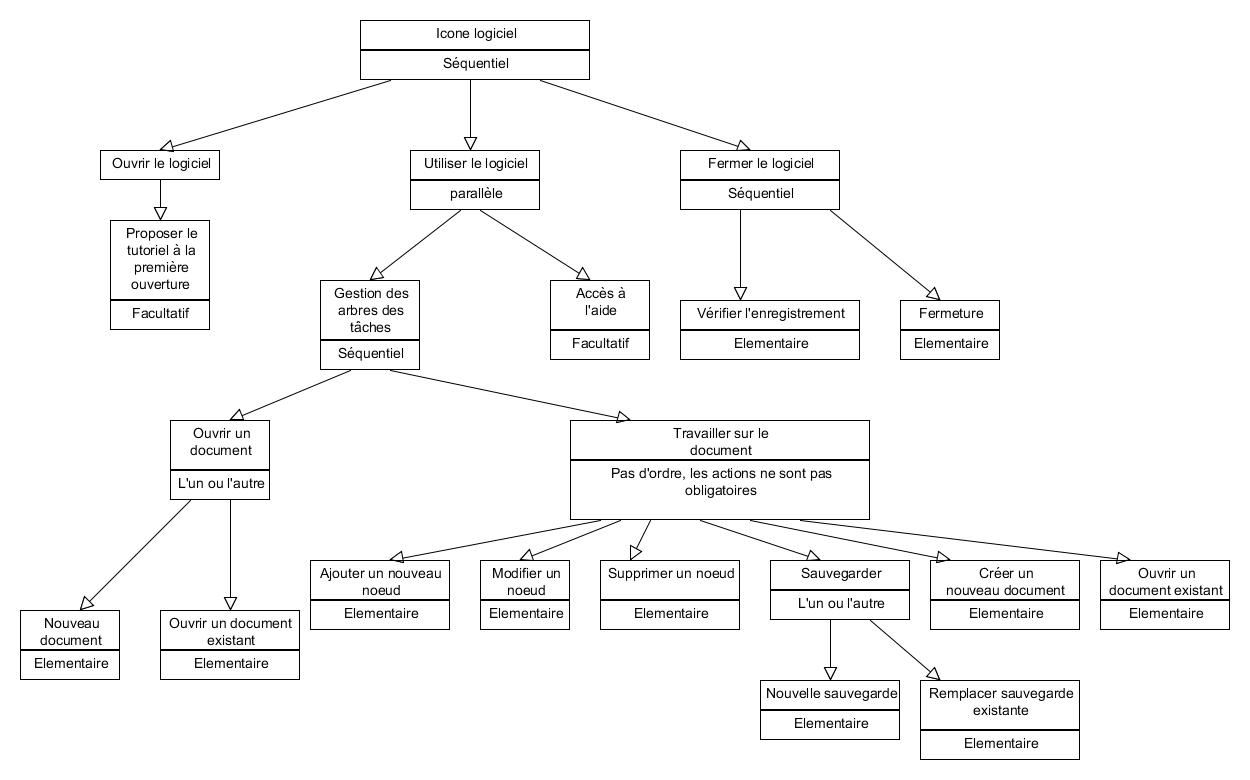
\includegraphics[scale = 0.4]{arbre-des-taches.jpg}
	\caption{L'arbre des tâches}
	\end{center}
\end{figure}


Explications supplémentaires : 
\begin{itemize}
\item [*]Au moment de cliquer sur \emph{nouveau document} lors d'une session de travail (travailler sur le document), l'arbre remonte jusqu'à travailler sur le document. De même au moment de cliquer sur \emph{Ouvrir un document existant}.
\item [*]La zone \emph{Travailler sur le document} ne comporte concrètement aucune contrainte, l'utilisateur peut faire ce qu'il souhaite (enregistrer un document vide est toujours possible par les menus), et certaines actions peuvent ne pas être effectuées (on peut par exemple créer un nœud, voire plusieurs, mais ne pas en supprimer).
\end{itemize}
\end{document}